\section{Objective 1: \texttt{mpbenchmark}}
As mentioned in the introduction section \texttt{mpbenchmark} performs calculations of a jet engine using multiple threads and produces the time taken to complete these calculations as output. The source code of \texttt{mpbenchmark} provided a solution in \texttt{C\#}\cite{mpbenchmark_code}, this served as a useful reference of how would be implemented in code using object-oriented design. Subsequently, the \texttt{C++} object oriented design comprised of three main classes:

\begin{enumerate}
	\item \texttt{FileDataLoader}: the primary function of this class is to load data from the input file and also to allow the user to save output data to the output file.
	\item \texttt{SharedPerformanceData}: this class stores data loaded from the input file into an array and also allows storage of output data into a separate array. But importantly it allows threads to access specific parts of the input data in a thread-safe manner. 
	\item \texttt{Worker}: this class contains functions to perform the important calculations, computations of deadlines missed and output data. This class defines the \texttt{operator ()} which encapsulates the main calculations, this class design is know as a \texttt{Functor}.
\end{enumerate}

The \texttt{C++} object-oriented class design can be visualised using a UML class diagram shown in figure \ref{fig:mpbenchmark_UML_diagram}.

\begin{figure}[H] % Positioning preference: here, top, bottom, page
	\centering
	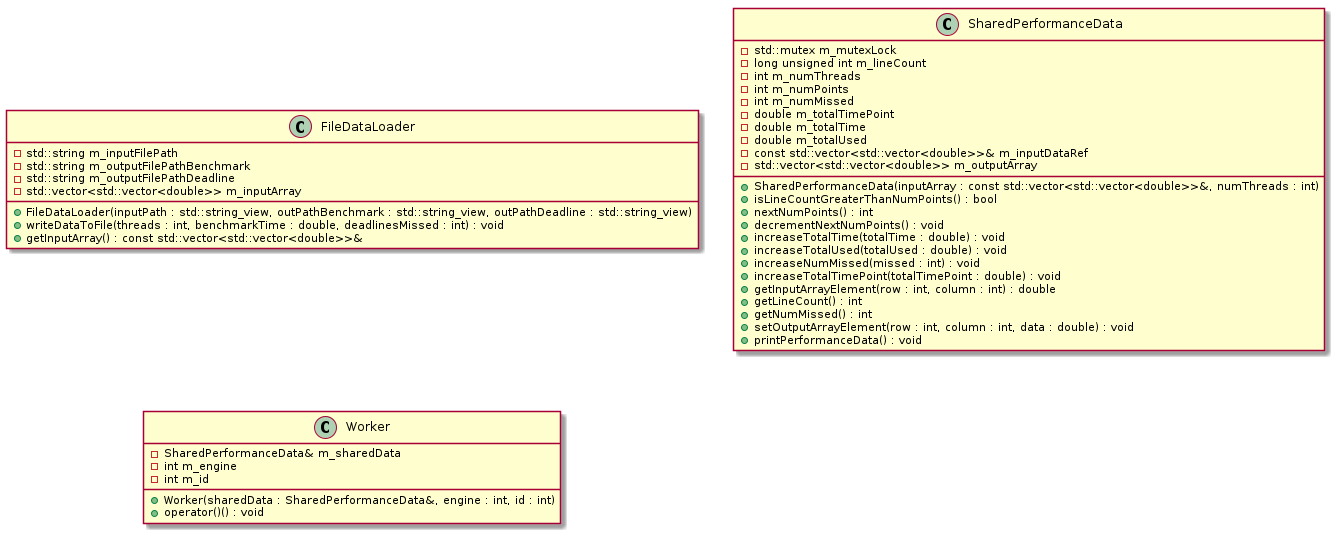
\includegraphics[width=1\textwidth, height=20cm]{~/Documents/Part_D_Modules/Individual_Project/Individual_report/figures/mpbenchmark_class.png} % Adjust the path and width as needed
	\caption{UML class diagram of the proposed \texttt{C++} solution.}
	\label{fig:mpbenchmark_UML_diagram} % Use this label to reference the figure
\end{figure}

The proposed solution employed the \texttt{fmt} library in \texttt{C++}\cite{fmt_printing_library} for output, providing an enhanced printing method compared to the \texttt{std::cout()} function from the \texttt{C++} standard library. Although the compiler on the target system supported the \texttt{C++20} standard, it lacked support for the \texttt{std::format()} function, which provides better printing capabilities in \texttt{C++}\cite{std_format_gcc_compiler_version}. Additionally, a new command line argument was introduced to adjust the number of threads used, complementing the existing argument that modifies the simulation engine. For compilation and linking, the industry-standard \texttt{CMake}\cite{cmake_about} software was utilized. In the \texttt{CMakeLists.txt} file, essential configurations included specifying the \texttt{C++20} standard, incorporating the \texttt{fmt} library, and compiling with the \texttt{-O2} optimization flag. This optimization flag, also used by the original authors of \texttt{mpbenchmark}\cite{mpbenchmark_paper}, was retained in the proposed solution for consistency.

An alternate solution was developed to further enhance the performance of \texttt{mpbenchmark}, the \texttt{Valgrind/Callgrind} function profiler tool was deployed to find potential bottlenecks. The application was compiled with debug information and optimisations turned off, this was done by specifying the build type as \texttt{Debug} and compiling with \texttt{-g} and \texttt{-O0} flags in the \texttt{CMake} file. \texttt{Callgrind} profiling results showed that part of the application where it approximates the value of $\pi$ had the highest self-cost. This code snippet is shown in the listing ~\ref{lst:pi_approximation_1} below:

\begin{lstlisting}[
	caption={Part of the code with the highest self-cost. It approximates $\pi$ using numerical integration.},
	label={lst:pi_approximation_1}
	]
// initialise variables for the pi calculation
const long num_steps = 1000000;
double step = 1.0 / static_cast<double>(num_steps);
double x{}, pi{}, sum{};

// performing numerical integration using the midpoint Riemann sum
for (int i = 0; i < num_steps; i++) {
	x = (i + 0.5) * step;
	sum += 4.0 / (1.0 + x * x);
}
pi = sum * step;
\end{lstlisting}

The problem with this part of the code was that it was already part of the parallel regions where it is executed by each thread. It may seen like a good candidate for applying parallel \texttt{for loop} from the OpenMP library however creating nested threads beyond the number of threads available on the system does not always lead to higher performance and in many cases can degrade performance. Another way to improve performance is by using SIMD intrinsics. An advantage of using \texttt{C++}(and/or \texttt{C}) is that SIMD intrinsics can be deployed whereas higher level languages like \texttt{Java} or \texttt{C\#} make it very difficult to access these. 

SIMD intrinsics vary by the target CPU, \texttt{x86} processors (which are found in most laptop and desktops) use \texttt{AVX2} instructions whereas \texttt{ARM} processors(commonly found in Apple products and embedded devices) use \texttt{NEON} instructions. In this project we use both as our proposed \texttt{C++} solution will be deployed on both desktop(\texttt{x86} processor) and Raspberry Pi devices(\texttt{ARM} based processor). The SIMD enhanced code can be summarised algorithmatically in the following steps and shown as a code snippet in listing ~\ref{lst:pi_approximation_2}: 

\begin{enumerate}
	\item Initialise \texttt{256-bit} wide vectors: each vector can hold four double-precision (\texttt{64-bit}) floating point numbers. The main initialisations would be a vector to hold four loop indices (\texttt{vec\_i}), a vector to calculate four values of $x$ (\texttt{vec\_x}), a vector to hold the result of the integrand (\texttt{vec\_temp}) and a vector to accumulate the sum (\texttt{vec\_sum}) after each loop iteration.
	\item \texttt{for loop} iterate until \texttt{num\_steps/4}:
	\begin{itemize}
		\item step 1: calculate the four midpoints $x$-values simultaneously using the vector \texttt{vec\_i} and hold result in \texttt{vec\_x}. Original formula used: \texttt{(i + 0.5) * step}.
		\item step 2: compute the value of the integrand in parallel using the four calculated $x$-values stored in \texttt{vec\_x}, store result in \texttt{vec\_temp}. Original formula used: \texttt{4 / (1 + x * x)}.
		\item step 3: accumulate the values from \texttt{vec\_temp} into the \texttt{vec\_sum} vector.
		\item step 4: increment loop indices vector \texttt{vec\_i} by \texttt{4}. 
	\end{itemize}
	\item Final summation: upon the completion of the loop, perform a horizontal sum on the vector (\texttt{vec\_sum}) that held the accumulated values.
	\item Calculation of $\pi$: sum is multiplied by the step size to approximate the value of $\pi$. Original formula used : \texttt{pi = sum * step}.
\end{enumerate}

The SIMD enhanced code implemented using \texttt{AVX2} instructions of listing ~\ref{lst:pi_approximation_1} is shown below in listing ~\ref{lst:pi_approximation_2}: 

\begin{lstlisting}[
	caption={SIMD enhanced code for approximation of $\pi$ using \texttt{AVX2} instructions. (Horizontal sum function in line 28 can be found in appendix).},
	label={lst:pi_approximation_2}
	]
double Worker::approximatePi(){
	double pi = 0.0; // Initialize pi to 0.0
	static constexpr long num_steps = 1000000; 
	static constexpr double step = 1.0 / static_cast<double>(num_steps); 
	
#if defined(__AVX2__)
	// Use AVX2 SIMD instructions if available
	double sum = 0; // Initialize scalar sum to accumulate final result
	
// Initialise all necessary 256-bit vectors
	__m256d vec_sum = _mm256_set1_pd(0.0);
	__m256d vec_step = _mm256_set1_pd(step);
	__m256d vec_half_step = _mm256_set1_pd(0.5 * step); 
	__m256d vec_one = _mm256_set1_pd(1.0); 
	__m256d vec_four = _mm256_set1_pd(4.0); 
	__m256d vec_x, vec_temp; 
	__m256d vec_i = _mm256_set_pd(3, 2, 1, 0); 
	__m256d vec_increment = _mm256_set1_pd(4); 

// Perform 4 computations at once, note "i" is incremented by 4 instead of 1
	for (int i = 0; i < num_steps; i += 4) {
		vec_x    = _mm256_add_pd(_mm256_mul_pd(vec_i, vec_step), vec_half_step); 
		vec_temp = _mm256_div_pd(vec_four, _mm256_add_pd(vec_one, _mm256_mul_pd(vec_x, vec_x))); 
		vec_sum  = _mm256_add_pd(vec_sum, vec_temp); 
		vec_i    = _mm256_add_pd(vec_i, vec_increment); 
	}
// Perform horizontal sum on vec_sum to get a scalar sum
	sum = hsum256_pd(vec_sum);
 // Multiply the sum by the step size to approximate pi
	pi = sum * step; 

#else
// If AVX2/SIMD instructions are unavailable then resort to using regular code... 
#endif

	return pi; 
}
\end{lstlisting}

As discussed, to utilize SIMD intrinsics on Raspberry Pi devices, \texttt{NEON} instructions must be employed. \texttt{NEON} instructions come with limitations, notably in their support for double precision floating points, which is restricted, and their vector width, which is only \texttt{128-bit}, compared to the \texttt{256-bit} vectors seen in \texttt{AVX2}\cite{neon_reference}. To accommodate \texttt{NEON}, two solutions were developed: one using single precision floating points (\texttt{float}) and the other using double precision floating points (\texttt{double}). The \texttt{NEON} code with \texttt{float} can perform four computations simultaneously, while the code with \texttt{double} can manage only two computations simultaneously, due to the \texttt{128-bit} vector's capacity to store four \texttt{float} values or two \texttt{double} values. Typically, \texttt{float} variables offer less decimal precision than \texttt{double} variables. These two SIMD-enhanced solutions, along with their decimal accuracy levels, will be compared in the results and discussion section. The \texttt{NEON} implementation follows the same algorithm as the code snippet shown in Listing~\ref{lst:pi_approximation_2}. The \texttt{CMake} also required some changes to allow the \texttt{AVX2} instructions to be used, this along with the \texttt{NEON} codes for Raspberry Pi can be found in the [Appendix Listings ~\ref{lst:cmake_simd}, ~\ref{lst:neon_float} and ~\ref{lst:neon_double}].

To collect benchmark data, the runtime was recorded and saved to a specified \texttt{.txt} file, the number of deadlines missed were also saved but in a separate \texttt{.txt} file. The application underwent 103 runs, with the first three designated as warm-up sessions; the subsequent 100 runs were averaged and utilized for plotting bar charts and speedup plots. For the languages \texttt{Java} and \texttt{C\#}, data were collected over 103 runs. In contrast, for the compiled languages \texttt{C}, \texttt{Ada}, and \texttt{C++}, the application was executed 203 times. The variance in the number of threads was controlled using the \texttt{taskset} command in Linux. Specifically for the \texttt{C++} application, a second command line argument was employed to specify the number of threads. This approach aligns with the methodology described by the authors of \texttt{mpbenchmark}\cite{mpbenchmark_paper}. An example bash script demonstrating how the application was executed multiple times is shown in the following listing (listing ~\ref{lst:benchmark_collection}):

\begin{lstlisting}[
	caption={Bash script to run application multiple times along with \texttt{taskset} command. Command line arguments: \texttt{mpbenchmark [engine\_type] [threads]} .},
	label={lst:benchmark_collection}
	]
# Loop to run the executable 103 times, using "3" as the default engine type and 2 cores/threads 
for i in {1..103}
do
	taskset -c 0,2 ./mpbenchmark 3 2 
done

# Loop to run the executable 103 times, using "3" as the default engine type and 4 cores/threads 
for i in {1..103}
do
	taskset -c 0,2,4,6 ./mpbenchmark 3 4 
done
\end{lstlisting}

The process of collecting benchmark times can be visualised in the image shown in figure ~\ref{fig:results_collection}. The python application used to plot the graphs was trivial and not shared in this report. The full system specification of the desktop and Raspberry Pi devices used to collect data can be found in the [Appendix ~\ref{tab:spec_comparisons}].

In summary, for desktop (\texttt{x86}) processors, two main solutions have been developed: a novel \texttt{C++} solution and a SIMD-enhanced \texttt{C++} solution as discussed in Listing~\ref{lst:pi_approximation_2}. For the Raspberry Pi devices, three solutions have been created: the first is the novel \texttt{C++} solution, identical to that on the desktop, and the other two are the SIMD-enhanced versions utilizing \texttt{NEON} instructions with single and double precision floating point variables.

\begin{figure}[htbp] % Positioning preference: here, top, bottom, page
	\centering
	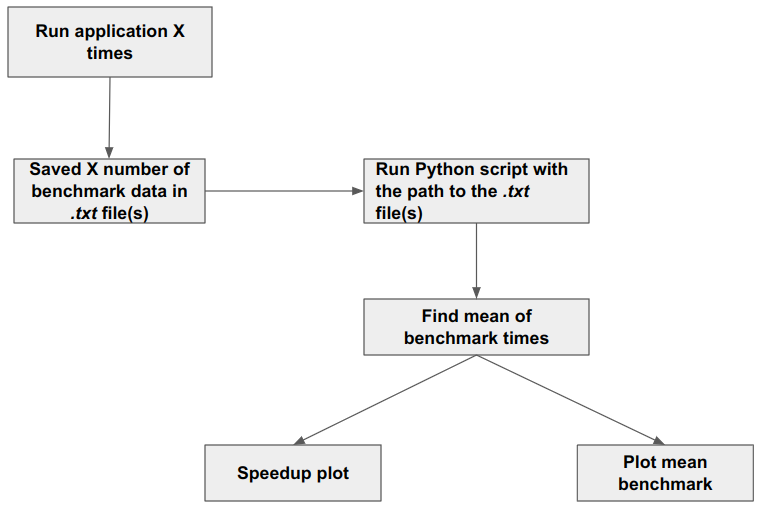
\includegraphics[width=0.5\textwidth]{~/Documents/Part_D_Modules/Individual_Project/Individual_report/figures/benchmarking_method.png} % Adjust the path and width as needed
	\caption{Benchmark results collection strategy.}
	\label{fig:results_collection} % Use this label to reference the figure
\end{figure}

\newpage
\section{Objective 2: \texttt{MobileNet}}
% Step 1: MobileNet setup
% Step 2: Valgrind results
% Step 3: OpenMP parallelisations and SIMD
% Step 4: Raspberry Pi different compilations

Setting up MobileNet from the \texttt{GitHub} repository\cite{mobilenet_repo} was a time consuming task. Details about the setting up process can be found in the [Appendix Listing ~\ref{lst:mobilenet_updates}]. Once setup the \texttt{MobileNet} project needed to be profiled with \texttt{Callgrind} function profiler to find bottlenecks and possible parallelisation points. To use \texttt{Callgrind}, the project was compiled with debug information and no optimisations. This required setting the build type as \texttt{Debug} and adding \texttt{-g} and \texttt{-O0} optimisation flags in the \texttt{CMakeLists.txt} file. \texttt{Callgrind} results showed that functions from the convolution and batch normalisation layer had the highest self-cost. The functions with the highest self-cost were \texttt{ConvLayer::forward()}, \texttt{BatchNormalLayer::forward()} and \texttt{ConvLayer::Addpad()}. The detailed \texttt{Calgrind} profiling results can be seen in [Appendix Figure ~\ref{fig:mobilenet_profiling}]. 

The CPU intensive function inside the convolution layer contained a number of nested \texttt{for} loops with large iterations. \texttt{OpenMP} library was used to parallelise the \texttt{for} loops. The \texttt{collapse} clause and dynamical scheduling type of the parallel \texttt{for} loop from the \texttt{OpenMP} library were implemented inside the \texttt{ConvLayer::forward()} function. To parallelise the other two functions \texttt{BatchNormalLayer::forward()} and \texttt{ConvLayer::Addpad()} only the \texttt{collapse} clause was utilised. The \texttt{ConvLayer::forward()} function contained some computations which were a good candidate for SIMD optimisations, these were more straight forward than compared to objective 1 as \texttt{OpenMP} library allows a simple way of using SIMD without the developer having to worry about \texttt{AVX2} or \texttt{NEON} instructions. 

For the Raspberry Pi processor it was decided to parallelise only the \texttt{ConvLayer::forward()}, \texttt{BatchNormalLayer::forward()} functions and not use the SIMD enhancements, as SIMD instruction's performance gains are more limited on embedded processors due to the narrower registers\cite{embedded_processors_reduced_simd_performance}. Having said that results from parallelising all the three functions and SIMD enhanced code were compared to find the optimal solution. This is discussed in the results and discussion section. 

To address the different compilations, the \texttt{CMake} file was altered. A macro \texttt{EMBEDDED\_PROC} was added. To compile the \texttt{MobileNet} project for \texttt{x86} processors the macro \texttt{EMBEDDED\_PROC} was set to \texttt{OFF}, this applies parallelisation to all three functions along with the SIMD enhancements. To compile the \texttt{MobileNet} project for Raspberry Pi processor the user can specify the \texttt{EMBEDDED\_PROC} to \texttt{ON}, this would parallelise only the two functions discussed and not apply SIMD enhancements. This can be seen in lines 15-18 in listing ~\ref{lst:mobilenet_parallel}. The parallelisation of the other two functions \texttt{BatchNormalLayer::forward()} and \texttt{ConvLayer::Addpad()} was very similar to \texttt{ConvLayer::forward} and can be found in [Appendix Listing ~\ref{lst:mobilenet_function1_parallel} and ~\ref{lst:mobilenet_function2_parallel}]. 

\begin{lstlisting}[
	caption={Parallelising the \texttt{ConvLayer::forward()} function and applying SIMD depending on the macro \texttt{EMBEDDED\_PROC}.},
	label={lst:mobilenet_parallel}
	]
void ConvLayer::forward(float *pfInput)
{
// collapse 3 "for" loops and use dynamic scheduling 
#pragma omp parallel for collapse(3) schedule(dynamic)
for (int g = 0; g < m_nGroup; g++)
{
	for (int nOutmapIndex = 0; nOutmapIndex < m_nOutputGroupNum; nOutmapIndex++)
	{
		for (int i = 0; i < m_nOutputWidth; i++)
		{
			
// other code to be ignored ... 
			
// Only use OpenMP SIMD optimizations if EMBEDDED_PROC is not defined 
			#ifndef EMBEDDED_PROC
			#pragma omp simd reduction(+:fSum)
			#endif
			for (int n = 0; n < m_nKernelWidth; n++)
			{
				nKernelIndex = nKernelStart + m * m_nKernelWidth + n;
				nInputIndex = nInputIndexStart + m * m_nInputPadWidth + n;
				fSum += m_pfInputPad[nInputIndex] * m_pfWeight[nKernelIndex];
			}
		}
	}              
}

}
\end{lstlisting}

In line 16 of the code snippet above(listing ~\ref{lst:mobilenet_parallel}) the reduction clause on the \texttt{fSum} was utilised to prevent race conditions. Moreover the arrays used must also be aligned to make full use of the SIMD clause. A 32-byte alignment was used for arrays \texttt{m\_pfInputPad} and  \texttt{m\_pfWeight}, this is shown in listing  ~\ref{lst:mobilenet_array_alignment}.

\begin{lstlisting}[
	caption={Making arrays that are 32-byte aligned for SIMD clause.},
	label={lst:mobilenet_array_alignment}
	]
ConvLayer::ConvLayer(/*Constructor arguments not shown ... */) 
{
// ignore other code ... 

// Creating arrays which are 32-byte aligned for SIMD optimisations 
size_t alignment = 32;
size_t inputPadSize = m_nInputNum * m_nInputPadWidth * m_nInputPadWidth * sizeof(float);
size_t weightSize   = m_nOutputNum * m_nInputGroupNum * m_nKernelSize * sizeof(float);
size_t outputSize   = m_nOutputNum * m_nOutputSize * sizeof(float);

m_pfInputPad = static_cast<float*>(aligned_alloc(alignment, inputPadSize));
m_pfWeight   = static_cast<float*>(aligned_alloc(alignment, weightSize));
}
\end{lstlisting}

The \texttt{MobileNet} application was designed with three command line arguments. The first argument determines whether to classify only one image or all images in the \texttt{data} folder. The second argument specifies whether the runtime should be saved to a \texttt{.txt} file, and the third sets the number of threads used. For data collection, the time taken to classify a single image was recorded while varying the number of threads. The number of threads utilized by the application was adjusted using the command line and \texttt{OpenMP}'s \texttt{omp\_set\_num\_threads()} function. Additionally, \texttt{MobileNet} includes an option to save the application's runtime to a designated \texttt{.txt} file. For benchmarking, the project was compiled with the \texttt{-O3} optimisation flag and was executed 103 times with different thread counts; the runtime and speedup plots were derived from the average of the 100 timing results stored in the \texttt{.txt} file. The method of data collection largely mirrors the process shown in figure~\ref{fig:results_collection}, with the exception that the \texttt{taskset} command was not employed to adjust the number of CPU cores; instead, thread adjustments were made through the command line. The detailed code snippet of the command line arguments can be found in the [Appendix Listing ~\ref{lst:mobilenet_command_line_arguments}].  

\section{Objective 3: \texttt{DeBaTE-FI} platform}
% Talk about profiling the application 
% C++ libraries for telnetpp and integration into the Debate-FI via Pybind-11
% Multi-processing and mutli-threaidng design improvement 

The application was profiled to find bottlenecks and possible points of optimisations. The tool \texttt{py-spy} was used to profile the application and save the output as a \texttt{.json} file\cite{py-spy}. The results were then viewed using the \texttt{speedscope} web application\cite{speedscope_app}. Since the application used multi-processing, the required processes were identified and their process \texttt{pid} was used to run \texttt{py-spy}, as shown below in Listing~\ref{lst:py_spy_application}:

\begin{lstlisting}[
	caption={Running \texttt{py-spy} on the specified process.},
	label={lst:py_spy_application}
	]
	py-spy record --pid <PID> --format speedscope -o profile.json 
\end{lstlisting}


Profiling results showed that the functions from \texttt{Python}'s \texttt{Telnetlib} library had the highest self-cost. To optimize the application, a \texttt{C++} open-source \texttt{Telnet} library was utilized. The \texttt{C++} library, called \texttt{telnetpp},\cite{telnetpp_library} along with \texttt{serverpp},\cite{serverpp_library} was integrated into the application using the tool \texttt{pybind11}. \texttt{pybind11} is a lightweight library for integrating \texttt{C++} into \texttt{Python} applications\cite{pybind11}. The \texttt{telnetpp} library required some functions for it to be integrated into the application; thus, a wrapper class in \texttt{C++} was created that allowed \texttt{telnetpp} to seamlessly replace the previous \texttt{telnetlib} \texttt{Python} library. The wrapper \texttt{C++} class was named \texttt{telnetlibcpp} for consistency. This \texttt{C++} class is shown in the following UML class diagram (Figure~\ref{fig:telnetlibcpp_UML}). The main functions used, \texttt{Readout()}, \texttt{Exec()}, and \texttt{write()}, have the exact same names as the functions from the \texttt{Python} library. Profiling results and detailed code snippet about the \texttt{C++} functions can be found in [Appendix ~\ref{sec:app_obj3}]. 

\begin{figure}[htbp] % Positioning preference: here, top, bottom, page
	\centering
	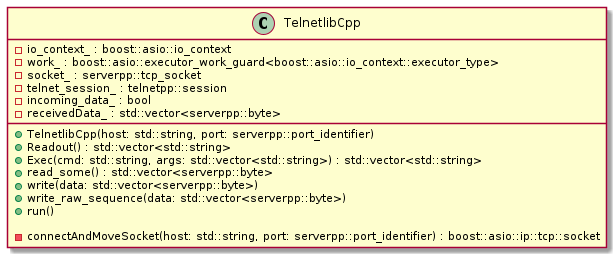
\includegraphics[width=1\textwidth, height=15cm]{~/Documents/Part_D_Modules/Individual_Project/Individual_report/figures/telnetlib_C++_class.png} % Adjust the path and width as needed
	\caption{\texttt{C++} class to emulate \texttt{Python's} \texttt{telnetlib} library functions.}
	\label{fig:telnetlibcpp_UML} % Use this label to reference the figure
\end{figure}

Using \texttt{CMake} and \texttt{pybind11} the \texttt{C++} class was compiled into a shared library(\texttt{.so}) file which was then moved into the same directory as the application. This allowed the \texttt{python} application to call the \texttt{C++} functions and use the \texttt{telnetpp} \texttt{C++} library. 

Another solution was developed which aimed to optimise the application's multi-processing and multi-threading. A simplified version of the application's architecture is shown below in the UML sequence diagram(Figure ~\ref{fig:original_application_arch}):

\begin{figure}[htbp] % Positioning preference: here, top, bottom, page
	\centering
	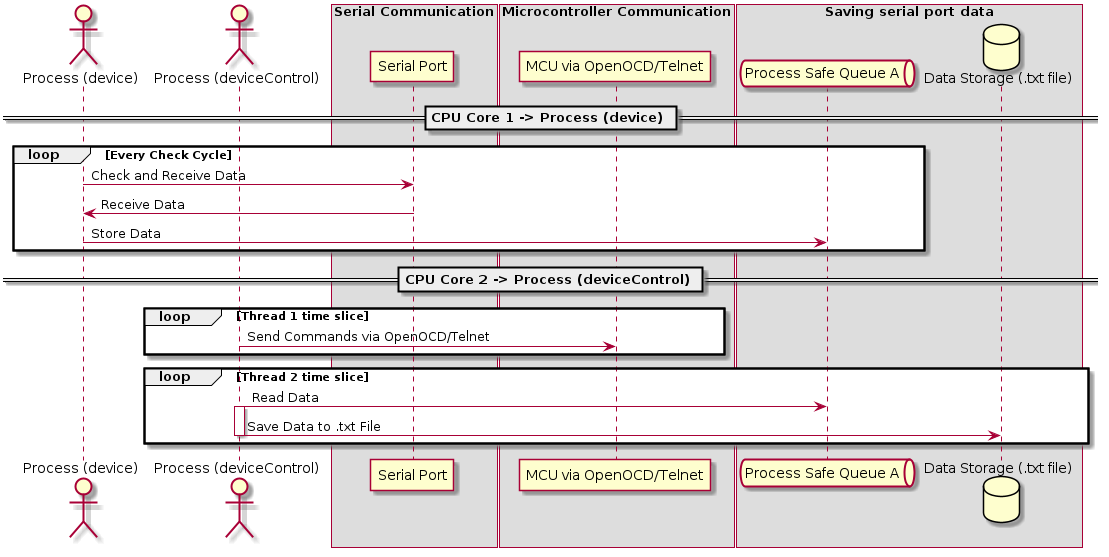
\includegraphics[width=1\textwidth, height=15cm]{~/Documents/Part_D_Modules/Individual_Project/Individual_report/figures/original_process_design.png} % Adjust the path and width as needed
	\caption{The sequence of the original application architecture. CPU Core 2 has to split CPU time between handling serial port data and sending commands.}
	\label{fig:original_application_arch} % Use this label to reference the figure
\end{figure}

Figure ~\ref{fig:original_application_arch} summarises how the original application had a convoluted design leading to poor performance:

\begin{enumerate}
	\item Two classes \texttt{device} and \texttt{deviceControl} spawned processes. 
	\item The \texttt{deviceControl} process had its workload split between sending commands to MCU and saving serial port data to \texttt{.txt} file.  
	\item The \texttt{device} process seem to be performing a redundant task of saving serial port data into a queue. 
\end{enumerate}

This design was improved as follows:

\begin{enumerate}
	\item Two classes \texttt{device} and \texttt{deviceControl} spawn processes with each having their own designated tasks.
	\item The \texttt{deviceControl} process now only sends data to the MCU.   
	\item The \texttt{device} process only focuses on receiving data from the serial port and saving it to the \texttt{.txt} file. 
\end{enumerate}

The key in the above improved design is removing the redundant work done as previously both of the processes were handling the serial port data. Handling serial port data does not require two processes it can be done using only one. When threads are used inside a process CPU time is split between the two threads. In the improved design both processes only perform one task and more importantly the \texttt{deviceControl} process has a reduced workload, this is important as the CPU time will be fully allocated to sending commands to the MCU . The challenge here was to make sure both of the processes were synchronised. This was accomplished using the \texttt{Event()} object from the \texttt{multiprocessing} \texttt{Python} library. When the \texttt{deviceControl} process started it sent a signal to the \texttt{device} process, to start checking and storing serial port data, and when the \texttt{deviceControl} process finished it sent a signal to stop the \texttt{device} process, stopping the \texttt{device} process would then save the accumulated serial port data into the \texttt{.txt} file. This can be visualised in the following UML sequence diagram (Figure ~\ref{fig:improved_application_design}):

\begin{figure}[htbp] % Positioning preference: here, top, bottom, page
	\centering
	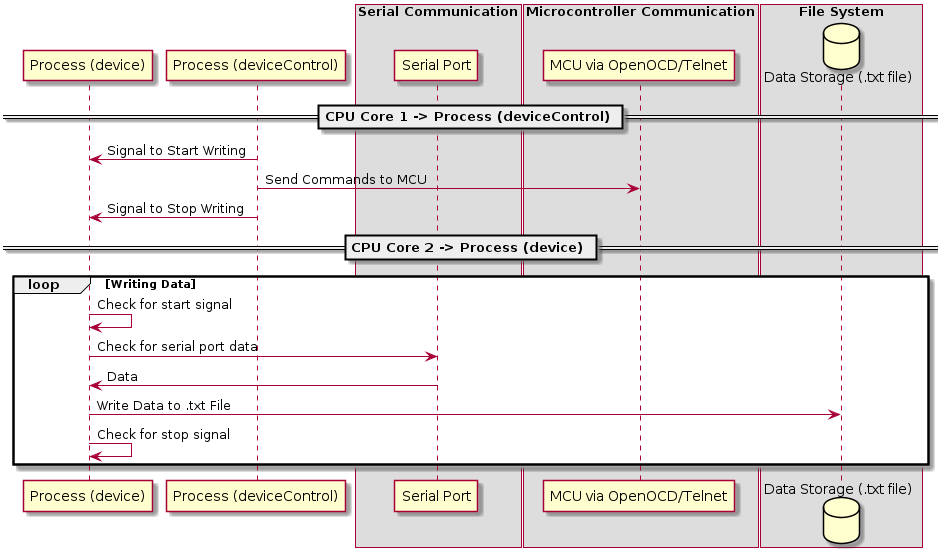
\includegraphics[width=1\textwidth, height=15cm]{~/Documents/Part_D_Modules/Individual_Project/Individual_report/figures/improved_process_design.png} % Adjust the path and width as needed
	\caption{The improved multi-processing design of the application. CPU Core 2 now allocates all the CPU time to sending commands to the MCU.}
	\label{fig:improved_application_design} % Use this label to reference the figure
\end{figure}

Results were collected using 4 \texttt{STM32F767ZI} MCUs for both of these solutions. In collaboration with Alex Henneman, results using the main setup(see figure ~\ref{fig:debate_fi_setup}) that utilised 36 MCUs running the second solution were also collected to verify the performance observed on the local setup. To collect benchmark data the application was run only once with varying number of boards and the run time was saved into a \texttt{.csv} file. The run time usually spanned in minutes thereby making multiple runs extremely time consuming, moreover the variation in run times was negligible unlike the applications in the first two objectives where the run times were in milliseconds and were more prone to variation. The benchmark collection strategy was similar to the one shown in figure ~\ref{fig:results_collection} except the application was run only once and the times were saved in a \texttt{.csv} file instead of a \texttt{.txt} file. 

\begin{figure}[htbp] % Positioning preference: here, top, bottom, page
	\centering
	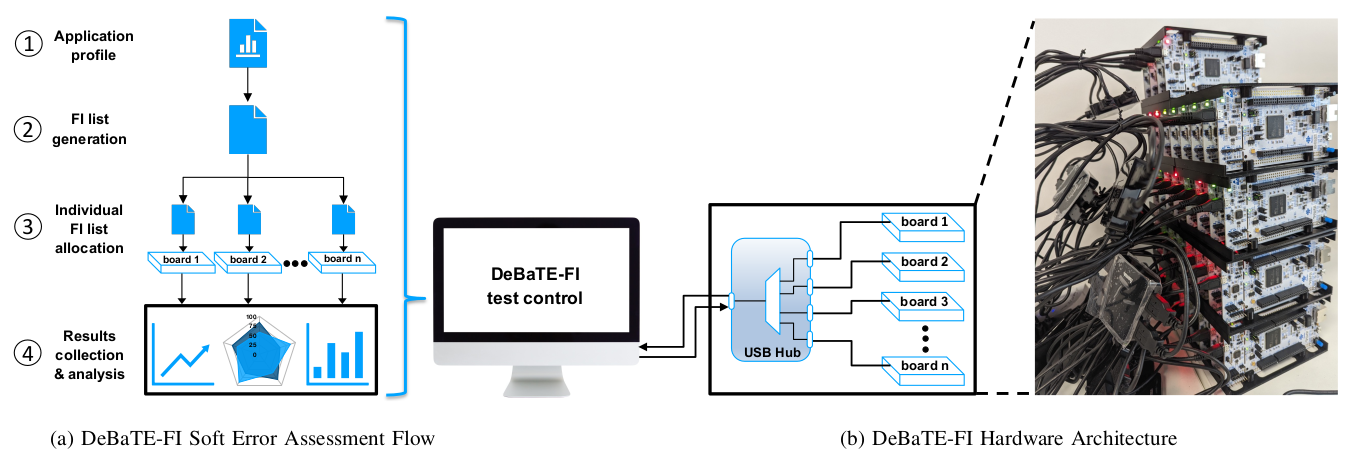
\includegraphics[width=1\textwidth, height=15cm]{~/Documents/Part_D_Modules/Individual_Project/Individual_report/figures/debate_fi_setup.png} % Adjust the path and width as needed
	\caption{\texttt{DeBaTE-FI} platform application on the main setup using 36 \texttt{STM32} boards\cite{debate_fi_publication}.}
	\label{fig:debate_fi_setup} % Use this label to reference the figure
\end{figure}